\section{Architettura}


\begin{frame}
\frametitle{Split an image into fixed-size patches}

Naive application of self-attention to images would require that \textbf{each pixel attends to every other pixel}. With \textbf{quadratic cost} in the number of pixels, this does \textbf{not scale to realistic input sizes} (even with very small images)

\begin{center}
    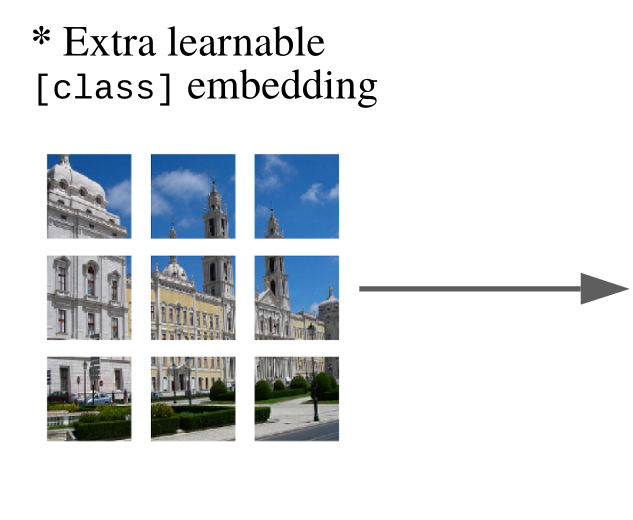
\includegraphics[width=0.5\textwidth]{img/2-section/Patching.png} 
\end{center}
\end{frame}

% \begin{frame}
% \frametitle{16x16 Patches}

%  ViT goes further to demonstrate that large scale pre-training makes \textbf{vanilla transformers competitive} with (or even better than) state-of-the-art CNNs. (Prior to this only 2x2 patches have been used)

% \begin{center}
%     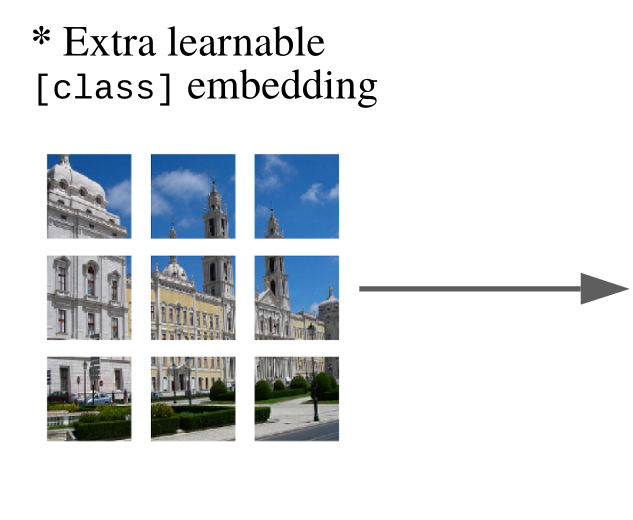
\includegraphics[width=0.5\textwidth]{img/2-section/Patching.png} 
% \end{center}
% \end{frame}


\begin{frame}
\frametitle{Position Embedding}

Positional Embedding provide information about the order of elements in a sequence, which is crucial for understanding \textbf{context}.

\vspace{0.5cm}

classification token token seves as as a global feature extractor that rappresents the entire image.

\begin{figure}[H]  % L'opzione [H] forza l'immagine a rimanere esattamente in quel punto nel testo
    \begin{center}
        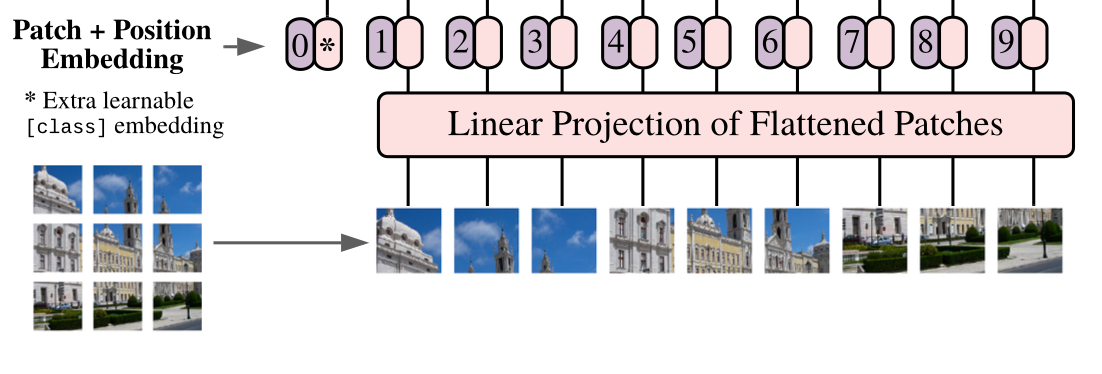
\includegraphics[width=0.8\textwidth]{img/2-section/Posizion enbedding.png}
        
    \end{center}
\end{figure}

\end{frame}

\begin{frame}
\frametitle{Transformer Encoding}


\begin{columns}
        \begin{column}{0.5\textwidth}
        Architecture of a Transformer:
            \begin{itemize}
            \item  Multi Head Attention
            \item Multi layer Perceptron (Feed Forward)
            \end{itemize}
        \end{column}
        \begin{column}{0.3\textwidth}
            \centering
            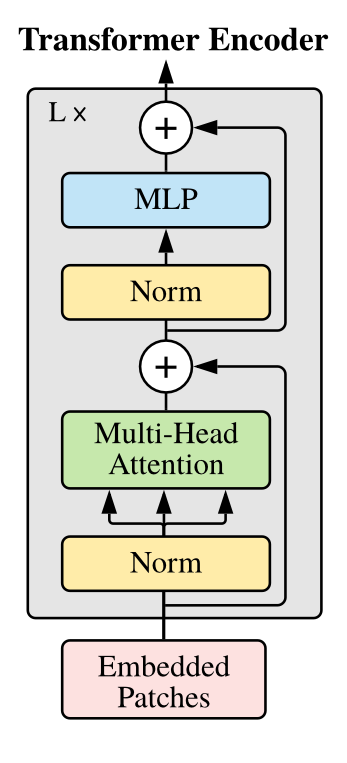
\includegraphics[width=\textwidth]{img/2-section/Transformer encoding.png}
        \end{column}
    \end{columns}


\end{frame}





\begin{frame}
\frametitle{Classification of the images}

After the last Transformer there is a MLP head that allow to classify each images.

\begin{center}
    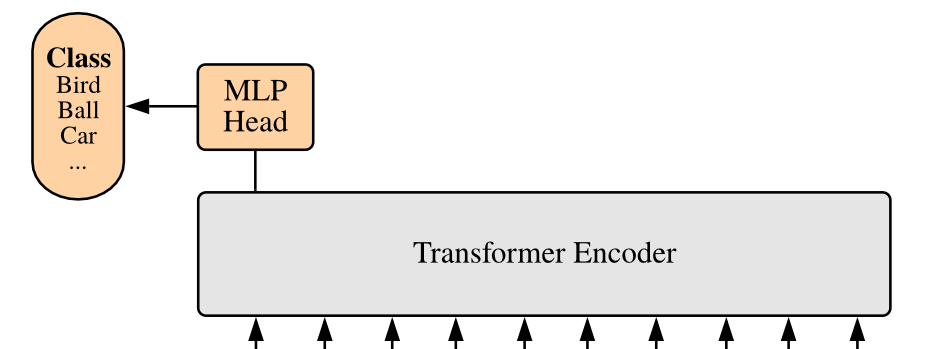
\includegraphics[width=0.8\textwidth]{img/2-section/Classification.png} 
\end{center}
\end{frame}